\documentclass[
  ngerman,
  DIV=14
]{scrartcl}
\usepackage{babel}
\usepackage{csquotes}

% typography
\usepackage{fontspec}
%\usepackage[utopia]{mathdesign}
\usepackage{newpxmath}
\setsansfont{Open Sans}[
  BoldFont={Open Sans Bold},
  ItalicFont={Open Sans Italic}]
\setmonofont[Scale=0.87]{Menlo}
\setmainfont{Palatino}
\linespread{1.15}
%\renewcommand\familydefault{\sfdefault}
\usepackage[factor=1000]{microtype}

% graphics, drawings, etc.
\usepackage{xcolor}
\usepackage{graphicx}
\usepackage[most]{tcolorbox}
\usepackage{tikz}
\usetikzlibrary{shapes.geometric}
\usetikzlibrary{shapes.arrows}
\usetikzlibrary{positioning}
\newtcolorbox{anmerkung}{%
  grow to left by=10pt,
  colback=black!10,
  colframe=white,
  coltitle=black,
  borderline west={4pt}{0pt}{black!30},
  boxrule=0pt,
  boxsep=0pt,
  %breakable,
  enhanced jigsaw,
  title={Anmerkung\par},
  fonttitle={\bfseries},
  attach title to upper={}}
\newtcolorbox{hinweis}{%
  grow to left by=10pt,
  colback=black!10,
  colframe=white,
  coltitle=black,
  borderline west={4pt}{0pt}{black!30},
  boxrule=0pt,
  boxsep=0pt,
  %breakable,
  enhanced jigsaw,
  title={Hinweis\par},
  fonttitle={\bfseries},
  attach title to upper={}}

% highlighting, lists, code
\usepackage{soul}
\usepackage{enumitem}
\usepackage{listings}
\lstset{
  basicstyle=\ttfamily,
  %escapeinside=||,
  keywordstyle=\color{blue!50!black},
  stringstyle=\color{green!50!black}}
\capsdef{////}{\scshape}{.16em}{.4em}{.2em}

% math
\usepackage{amsmath}

% nice tables
\usepackage{booktabs}
\newcommand{\tablespacing}[1]{\renewcommand{\arraystretch}{#1}}

% links
\usepackage[
  colorlinks,
  linkcolor={red!50!black},
  citecolor={blue!50!black},
  urlcolor={blue!80!black}
]{hyperref}

\title{Lösungsblatt Nr. 1}
\date{Wintersemester 2018-2019}
\author{Andreas Koch}
\subject{Einführung in den Compilerbau}
\subtitle{Patrick Elsen, Viola Hofmeister und Michael Matthé}
\publishers{Technische Universität Darmstadt}

\begin{document}
\maketitle

\subsection*{Einleitung}

Auf diesem Aufgabenblatt sollen Sie sich mit der \emph{Matrix and Vector Language}, kurz MAVL, vertraut machen. Studieren Sie bitte zunächst die MAVL-Sprachspezifikation, die Sie im Moodle-Kurs der Veranstaltung finden.

\subsection*{Aufgabe 1.1: MAVL-Syntax}

Die MAVL-Sprachspezifikation enthält nur eine informelle Beschreibung der Syntaxelemente der Sprache. In den folgenden Teilaufgaben sollen Sie einige der Syntaxelemente in Produktionen einer kontextfreien Grammatik überführen.

\subsection*{Aufgabe 1.1a: Produktionen}

\emph{Geben Sie Produktionen für die Nichtterminale \texttt{mulExpr} (Multiplikations-Operator), \texttt{subvectorExpr} (Subvektor-Operator), sowie \texttt{recordElementSelectExpr} (Selektion von Record-Elementen) an.}

\bigskip\noindent
Ein Multiplikationsausdruck ist in der Sprachspezifikation unter \emph{§~7.5 Ternärer Operator} definiert. Ein solcher Ausdruck nimmt \verb|int| oder \verb|float|-Ausdrücke als Parameter und ist Linksassoziativ. Also kann man diesen grammatikalisch folgendermaßen definieren. 
\begin{lstlisting}
mulExpr ::= expr '*' expr
\end{lstlisting}
Die \verb|subvectorExpr| ist in dem Sprachstandard unter \emph{§~7.7.4 Submatrix und Subvektor} definiert. Hier wird definiert, dass eine solche Beispielsweise als $v\{l:e:u\}$ geschrieben werden kann, wobei $v$ ein Vektor, $e$ eine \texttt{int}-Ausdruck, und $l$ und $u$ konstante \texttt{int}-Ausdrücke sein müssen, so dass $l < u$. Dieser Ausdruck extrahiert einen Subvektor mit den Elementen $[i+l, i+u]$. Zuerst brauchen wir also ein Hilfs-Nichtterminalsymbol \texttt{constExpr} für $l$ und $u$.
\begin{lstlisting}
constExpr ::= '-'? INT (('*' | '+' | '-' | '/' | '^') constExpr)?
            | '(' constExpr ')'
\end{lstlisting}
Mit diesem Hilfsausdruck können wir nun die \texttt{subvectorExpr} definieren. Da $e$ ein beliebiger Ausdruck sein kann, können wir hier eine \texttt{expr} verwenden. 
\begin{lstlisting}
subvectorExpr ::= expr '{' constExpr ':' expr ':' constExpr '}'  
\end{lstlisting}
Unter \emph{§~7.8 Selektion von Record-Elementen} ist definiert, wie der Syntax der Recordelementselektion funktioniert. Mit diesem kann man auf ein bestimmtes Element eines Records zugreifen. Mit dem Ausdruck \texttt{person@name} greift man zum Beispiel auf das Namenselement des Records \texttt{person} zu. 
\begin{lstlisting}
recordElementSelectExpr ::= expr '@' ID  
\end{lstlisting}

\subsection*{Aufgabe 1.1b}

\emph{Geben Sie Produktionen für die Nichtterminale \texttt{primitiveType} (primitive Typen) und \texttt{vectorType} (Vektortypen) an.}

\bigskip\noindent
Die primitiven Typen sind unter \emph{§~4.2 Primitive Datentypen} definiert. Hier sind nur \texttt{int}, \texttt{float} und \texttt{bool} als eingebaute, primitive Typen angegeben. Also könnte eine Grammatik folgendermaßen aussehen:
\begin{lstlisting}
primitiveType ::= 'int' | 'float' | 'bool'
\end{lstlisting}
Der \texttt{vectorType} ist bei \emph{§~4.5 Vektoren} definiert. Ein Vektor muss, mit einem Elementtyp (entweder \texttt{int} oder \texttt{float}) und einer Länge (positive, ganze Zahl) definiert werden. Die Länge muss ein konstanter Ausdruck sein, also können wir hier wieder \texttt{constExpr} benutzen.
\begin{lstlisting}
vectorType ::= 'vector' '<' ('int' | 'float') '>' '[' constExpr ']'
\end{lstlisting}

\subsection*{Aufgabe 1.1c}

\emph{Geben Sie Produktionen für die Nichtterminale \texttt{returnStmt} (Rückgabebefehl), \texttt{varDecl} Variablendeklaration), \texttt{callStmt} (Aufruf-Befehl, ohne Rückgabewert) sowie \texttt{forStmt} (For-Schleife) an.}

\bigskip\noindent
Der Rückgabebefehl ist unter \emph{§~6.8 Rückgabe} im Sprachstandard definiert. Ein solcher Befehl besteht aus dem Keyword \texttt{'return'}, einem Ausdruck und einem abschließenden Semikolon. Also kann man einen solchen folgendermaßen definieren.
\begin{lstlisting}
returnStmt ::= 'return' expr ';'
\end{lstlisting}
Die Variablendeklaration ist unter \emph{§~6.2 Variablendeklaration} im Sprachstandard definiert. Eine solche Deklaration besteht aus dem Keyword \texttt{var}, dem Typen der Variablen (primitiver Typ wie \texttt{int}, \texttt{float} oder \texttt{bool}, Vektor, Matrix oder Record), sowie ein Variablenname.
\begin{lstlisting}
varDecl ::= 'var' (primitiveType | vectorType | matrixType | ID) ID ';'  
\end{lstlisting}
Aufrufe sind unter \emph{§~6.4 Aufrufe} im Sprachstandard definiert. Diese bestehen aus dem Namen einer Funktion, einer Klammer \texttt{'('}, den Parametern (durch Kommata separiert) und einer Klammer \texttt{')'}.
\begin{lstlisting}
callStmt ::= ID '(' (expr (',' expr)*)? ')' ';'
\end{lstlisting}
Die For-Schleife ist unter \emph{§~6.6.1 For-Schleife} definiert. Es besteht aus dem Keyword \texttt{for}, einer offenen Klammer, einer initialen Zuweisung, einer Kondition (boolscher Ausdruck, der bei jedem Durchlauf ausgewertet wird), eine Zuweisung, die nach jeden Durchlauf ausgeführt wird (typischerweise, um eine Zählervariable zu inkrementieren), eine schließende Klammer, sowie entweder ein einzelner Ausdruck oder mehrere Ausdrücke in geschweiften Klammern. Daraus ergibt sich folgende Grammatik.
\begin{lstlisting}
forStmt ::= 'for' '(' ID '=' expr ';' expr ';' ID '=' expr ')'
            (statement | '{' statement* '}')
\end{lstlisting}

\subsection*{Aufgabe 1.2: AST zu MAVL}
Abstrakte Syntaxbäume (engl. \emph{Abstract Syntax Tree}) sind eine weitverbreitete Zwischendarstellung, die nur essentielle Informationen enthält und Details der konkreten Syntax einer Programmiersprache abstrahiert. In dieser Aufgabe zeigen wir Ihnen eine mögliche Repräsentation von MAVL-Code als AST. Die darin verwendeten AST-Knoten korrespondieren auf natürliche Weise mit den in der Spezifikation beschriebenen Syntaxelementen. 

\subsection*{Artikel 1.2a}
\emph{Geben Sie den zum AST zugehörigen MAVL-Code an.}  

\bigskip\noindent
\begin{lstlisting}
if(flag & r > q) {
  r = -1;
  e(q, r);
} else {
  r = a - (q * d);
}
\end{lstlisting}

\subsection*{Artikel 1.2b}
\emph{Geben Sie den zum AST zugehörigen MAVL-Code an.}

\bigskip\noindent
\begin{lstlisting}
var vector<int>[3 + 1] p;
foreach(var int i : p) {
  i = k;
}  
\end{lstlisting}


\subsection*{Artikel 1.3: Ausdrücke}
Ausdrücke in typischen Programmiersprachen lassen sich einfach durch mehrdeutige Grammatiken beschreiben, die aber als Grundlage für die syntaktische Analyse ungeeignet sind.

\subsection*{Artikel 1.3a}
\emph{Zeichnen Sie den AST für den MAVL-Ausdruck \texttt{q \& a == b \# c}.}


\bigskip\noindent
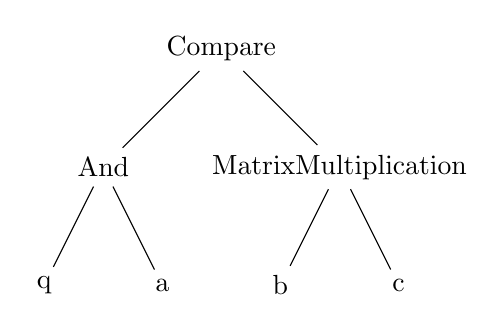
\begin{tikzpicture}[level distance=1.5cm,
level 1/.style={sibling distance=3cm},
level 2/.style={sibling distance=1.5cm}
]
\node{Compare}
child {node {And}
	child {node {q}}
	child {node {a}}
}
child {node {MatrixMultiplication}
	child {node {b}}
	child {node {c}}
};
\end{tikzpicture}


\subsection*{Artikel 1.3b}
\emph{Zeichnen Sie den AST für den MAVL-Ausdruck\texttt{ - v2 .* v1 + (v2 \# m)[0]}.}


\bigskip\noindent
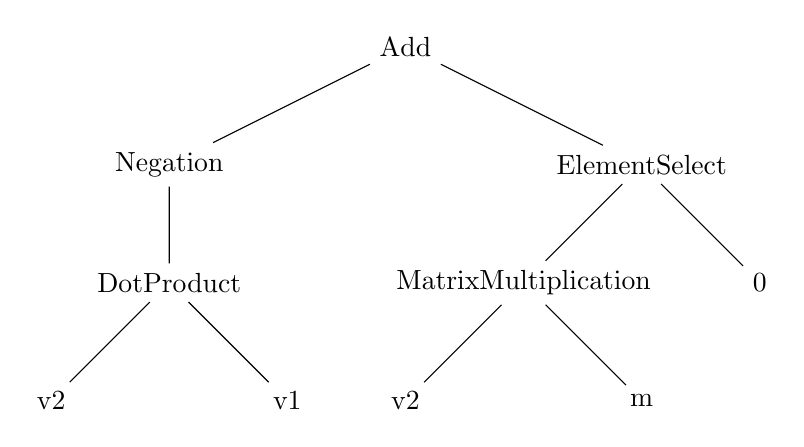
\begin{tikzpicture}[level distance=1.5cm,
level 1/.style={sibling distance=6cm},
level 2/.style={sibling distance=3cm}
]
\node{Add}
child {node {Negation}
	child {node {DotProduct}
		child {node {v2}}
		child {node {v1}}		
	}
}
child {node {ElementSelect}
	child {node {MatrixMultiplication}
		child {node {v2}}
		child {node {m}}
	}
	child {node {0}}
};

\end{tikzpicture}

\subsection*{Aufgabe 1.3c}
\emph{Gegeben seien folgende Wertedefinitionen.}
\begin{lstlisting}
val matrix <int>[2][2] m = [[1, 2],
                            [3, 4]];
val vector<int>[2]    v1 = [4, 2];
val vector<int>[2]    v2 = [2, 3];
\end{lstlisting}
\emph{Welchen Wert liefert der Ausdruck aus Teilaufgabe 1.3b?}

\bigskip\noindent
Dieses Programm kann man als ein kleines Ruby-Skript ausdrücken, was (hoffentlich) das richtige Ergebnis liefert. Wichtig ist hier, dass Ruby andere Operatopräzedenzregeln hat, weswegen anders geklammert werden muss.
\begin{lstlisting}[language=ruby,morekeywords={require,puts}]
require "matrix"
\end{lstlisting}
\begin{lstlisting}[language=ruby,morekeywords={require,puts}]
m = Matrix[[1, 2], [3, 4]]
v1 = Vector[4, 2]
v2 = Vector[2, 3]
\end{lstlisting}
\begin{lstlisting}[language=ruby,morekeywords={require,puts}]
puts (-v1.inner_product(v2) + (v2.covector * m)[0,0])  
\end{lstlisting}
Dieses Programm liefert als Resultat der Berechnung das Ergebis \texttt{-3}. 

\end{document}